\documentclass[a4paper]{article}

\usepackage{url}
\usepackage{graphicx}
\usepackage{enumerate}
\usepackage{amsmath}
\usepackage{float}
\usepackage{longtable}
\usepackage{fullpage}
\usepackage{pstricks}
\usepackage{tikz}
\usepackage[absolute]{textpos}

\title{
    \vspace{5cm}
    \huge{G53IDS Individual Dissertation Single Honours} \\[0.5cm]
    \LARGE{Project Proposal} \\[0.2cm]
}
\author{Robert J. Golding (rjg08u)} \date{\today}

\begin{document}
    \begin{textblock*}{60mm}(145mm,10mm)
        %LaTeX with PSTricks extensions
%%Creator: inkscape 0.47
%%Please note this file requires PSTricks extensions
%\psset{xunit=.5pt,yunit=.5pt,runit=.5pt}
\psset{xunit=0.25pt,yunit=0.25pt}
\begin{pspicture}(570.14807129,168.19282532)
{
\newrgbcolor{curcolor}{0.05098039 0.43529412 0.54901963}
\pscustom[linestyle=none,fillstyle=solid,fillcolor=curcolor]
{
\newpath
\moveto(148.216066,84.09640532)
\curveto(148.216066,167.87061532)(148.220066,168.19282532)(149.182696,168.19282532)
\curveto(150.145616,168.19282532)(150.149316,167.87061532)(150.149316,84.09640532)
\curveto(150.149316,0.32223532)(150.145316,0.00000532)(149.182696,0.00000532)
\curveto(148.219766,0.00000532)(148.216066,0.32223532)(148.216066,84.09640532)
\closepath
\moveto(72.094306,9.38182532)
\curveto(67.052806,10.35734532)(63.279006,11.76450532)(54.453396,15.95980532)
\curveto(44.430606,20.72415532)(40.674686,21.77159532)(32.462666,22.09251532)
\curveto(22.470056,22.48303532)(14.700625,20.76340532)(5.155495,16.04849532)
\curveto(2.630185,14.80111532)(0.356575,13.69186532)(0.103015,13.58350532)
\curveto(-0.636715,13.26741532)(2.757125,17.38818532)(5.494605,20.12997532)
\curveto(12.968645,27.61571532)(21.542856,30.92225532)(33.496726,30.92862532)
\curveto(44.058216,30.93462532)(50.857706,29.21134532)(63.255586,23.38808532)
\curveto(72.553376,19.02091532)(76.605636,17.63313532)(82.243876,16.88506532)
\curveto(92.104476,15.57673532)(101.993206,17.82868532)(109.235686,23.03188532)
\lineto(111.706796,24.80718532)
\lineto(109.676866,22.38264532)
\curveto(105.121066,16.94126532)(98.546116,12.47705532)(91.910136,10.31954532)
\curveto(87.149816,8.77183532)(77.585616,8.31926532)(72.094306,9.38182532)
\closepath
\moveto(399.780346,14.70082532)
\curveto(396.372396,15.48253532)(392.672346,16.90308532)(392.873036,17.35276532)
\curveto(392.950536,17.52641532)(393.536596,18.89660532)(394.175356,20.39758532)
\lineto(395.336746,23.12660532)
\lineto(397.800196,22.10343532)
\curveto(399.757796,21.29035532)(401.312756,21.07451532)(405.372646,21.05218532)
\curveto(410.119366,21.02608532)(410.619496,21.11528532)(412.425966,22.31010532)
\curveto(414.798486,23.87927532)(415.989066,26.25028532)(416.338276,30.10142532)
\curveto(416.601166,33.00069532)(416.596246,33.01478532)(415.441166,32.66789532)
\curveto(414.802376,32.47604532)(412.613326,32.07976532)(410.576616,31.78724532)
\curveto(398.936396,30.11549532)(391.189656,37.71202532)(390.501816,51.47279532)
\curveto(389.726716,66.97927532)(397.447176,75.93652532)(411.524466,75.86322532)
\curveto(415.398136,75.84302532)(421.308046,74.84399532)(423.846496,73.78019532)
\lineto(425.680266,73.01170532)
\lineto(425.538086,49.19281532)
\lineto(425.395916,25.37391532)
\lineto(424.241876,23.04976532)
\curveto(422.574566,19.69189532)(419.363176,16.69154532)(416.086666,15.43048532)
\curveto(412.568176,14.07628532)(404.146146,13.69940532)(399.780346,14.70082532)
\closepath
\moveto(415.125526,38.69643532)
\lineto(416.454636,39.30348532)
\lineto(416.454636,54.18996532)
\lineto(416.454636,69.07645532)
\lineto(414.405556,69.62821532)
\curveto(413.278566,69.93168532)(411.426146,70.05245532)(410.289066,69.89660532)
\curveto(404.094786,69.04758532)(401.121706,64.53776532)(400.629936,55.24482532)
\curveto(400.245756,47.98486532)(401.582636,42.39513532)(404.288386,39.94816532)
\curveto(406.674206,37.79053532)(411.836606,37.19426532)(415.125526,38.69643532)
\closepath
\moveto(62.186396,30.17547532)
\curveto(47.959166,37.47806532)(31.805996,38.20666532)(19.596306,32.09653532)
\lineto(17.362825,30.97882532)
\lineto(16.333945,32.07401532)
\curveto(15.341155,33.13079532)(15.305065,33.59155532)(15.305065,45.20875532)
\lineto(15.305065,57.24829532)
\lineto(18.530766,60.49891532)
\lineto(21.756486,63.74952532)
\lineto(22.949906,83.87250532)
\lineto(24.143336,103.99548532)
\lineto(19.965856,108.19240532)
\lineto(15.788375,112.38932532)
\lineto(15.788375,130.37239532)
\lineto(15.788375,148.35545532)
\lineto(20.259016,150.51905532)
\curveto(24.596986,152.61845532)(31.083736,155.15336532)(33.791776,155.80741532)
\lineto(35.120886,156.12842532)
\lineto(35.120886,147.74179532)
\curveto(35.120886,143.12914532)(35.242006,139.23405532)(35.390036,139.08601532)
\curveto(35.538066,138.93798532)(36.788636,139.10091532)(38.169086,139.44806532)
\curveto(39.549526,139.79521532)(42.255786,140.33471532)(44.182996,140.64695532)
\lineto(47.687016,141.21464532)
\lineto(47.687016,149.86140532)
\lineto(47.687016,158.50815532)
\lineto(49.016126,158.86186532)
\curveto(50.836706,159.34637532)(69.617166,159.34443532)(72.456796,158.85986532)
\lineto(74.752526,158.46776532)
\lineto(74.752526,149.29926532)
\curveto(74.752526,142.38102532)(74.900806,140.08735532)(75.356676,139.95387532)
\curveto(75.688946,139.85657532)(78.312856,139.41585532)(81.187576,138.97449532)
\curveto(86.953946,138.08915532)(93.781616,136.18805532)(100.685936,133.54535532)
\lineto(105.201236,131.81705532)
\lineto(105.201236,120.99783532)
\lineto(105.201236,110.17861532)
\lineto(101.752456,106.92480532)
\curveto(96.724186,102.18078532)(97.047836,102.32683532)(93.935896,103.39750532)
\curveto(88.156426,105.38593532)(83.504746,106.04575532)(75.116056,106.06702532)
\curveto(70.046606,106.07982532)(67.026466,106.26816532)(67.034606,106.57086532)
\curveto(67.041606,106.83668532)(67.692396,109.33782532)(68.480476,112.12895532)
\curveto(69.268566,114.92008532)(69.909916,117.42123532)(69.905686,117.68705532)
\curveto(69.901686,117.95287532)(68.057236,115.34298532)(65.807416,111.88730532)
\lineto(61.716846,105.60423532)
\lineto(61.709846,84.61021532)
\lineto(61.702846,63.61618532)
\lineto(63.877756,60.84787532)
\lineto(66.052656,58.07956532)
\lineto(66.052656,43.29770532)
\curveto(66.052656,35.16768532)(65.889546,28.52655532)(65.690176,28.53962532)
\curveto(65.490806,28.55272532)(63.914006,29.28901532)(62.186156,30.17588532)
\closepath
\moveto(44.303826,69.78418532)
\curveto(44.303826,71.74786532)(44.073686,78.87068532)(43.792406,85.61267532)
\curveto(43.222746,99.26642532)(43.033026,100.05127532)(40.305356,100.03832532)
\curveto(36.941776,100.02242532)(36.731356,99.27245532)(36.374536,86.02966532)
\curveto(36.206226,79.78284532)(35.940956,72.76876532)(35.785046,70.44282532)
\lineto(35.501586,66.21383532)
\lineto(39.902706,66.21383532)
\lineto(44.303826,66.21383532)
\lineto(44.303826,69.78418532)
\closepath
\moveto(485.626736,30.99352532)
\curveto(480.211326,31.89299532)(476.077806,34.73896532)(474.138646,38.90315532)
\curveto(472.862026,41.64456532)(472.570996,47.40516532)(473.562196,50.31322532)
\curveto(475.900706,57.17416532)(482.707916,60.77415532)(492.455226,60.30478532)
\lineto(497.167856,60.07785532)
\lineto(497.167856,62.19474532)
\curveto(497.167856,67.59657532)(494.126616,69.89811532)(487.543506,69.47819532)
\curveto(485.526786,69.34954532)(482.503086,68.75804532)(480.824146,68.16373532)
\curveto(479.145206,67.56942532)(477.716166,67.15943532)(477.648486,67.25264532)
\curveto(477.580786,67.34584532)(477.068426,68.64766532)(476.509856,70.14555532)
\lineto(475.494266,72.86899532)
\lineto(478.591986,73.88590532)
\curveto(485.616206,76.19179532)(493.996076,76.41597532)(498.517466,74.41894532)
\curveto(501.257456,73.20874532)(503.649516,71.00534532)(505.064026,68.38874532)
\curveto(506.067536,66.53250532)(506.114946,65.80261532)(506.254186,50.06636532)
\curveto(506.369696,37.02073532)(506.271086,33.59589532)(505.770876,33.27853532)
\curveto(503.794856,32.02473532)(494.823556,30.39682532)(490.487316,30.50519532)
\curveto(489.243896,30.53629532)(487.056616,30.75601532)(485.626736,30.99352532)
\closepath
\moveto(495.717926,36.72387532)
\lineto(496.926206,37.04215532)
\lineto(497.057806,45.79212532)
\lineto(497.189366,54.54208532)
\lineto(494.499056,54.87822532)
\curveto(486.495396,55.87820532)(482.361326,52.32155532)(482.742956,44.76417532)
\curveto(482.892296,41.80675532)(483.139366,40.94745532)(484.264426,39.47239532)
\curveto(486.801816,36.14571532)(490.318936,35.30170532)(495.717926,36.72387532)
\closepath
\moveto(252.796966,31.58349532)
\curveto(243.897516,33.85426532)(239.390066,41.19108532)(239.390066,53.40605532)
\curveto(239.390066,62.05380532)(241.417306,67.69905532)(246.003496,71.82243532)
\curveto(250.581506,75.93846532)(258.925096,77.07388532)(265.093586,74.42028532)
\curveto(268.435226,72.98274532)(272.366876,68.73443532)(273.784866,65.02902532)
\curveto(276.900156,56.88825532)(276.190546,45.00897532)(272.212546,38.70740532)
\curveto(270.540566,36.05882532)(266.907756,33.05190532)(264.305136,32.16236532)
\curveto(261.167266,31.08988532)(255.791296,30.81946532)(252.796966,31.58349532)
\closepath
\moveto(261.752716,38.07599532)
\curveto(264.974576,40.47724532)(266.352956,46.07466532)(266.003846,55.33930532)
\curveto(265.644606,64.87294532)(263.510676,69.32917532)(259.015906,69.93204532)
\curveto(253.259596,70.70413532)(250.195056,64.98756532)(250.195056,53.47770532)
\curveto(250.195056,44.70594532)(251.611336,40.11642532)(255.035536,37.79191532)
\curveto(257.015746,36.44765532)(259.721416,36.56207532)(261.752716,38.07599532)
\closepath
\moveto(290.134696,32.12328532)
\curveto(289.107886,32.48932532)(287.620416,33.40411532)(286.829176,34.15614532)
\curveto(283.804486,37.03100532)(283.807686,37.01199532)(283.543626,53.64770532)
\lineto(283.301976,68.87205532)
\lineto(281.006236,69.01936532)
\lineto(278.710506,69.16667532)
\lineto(278.710506,72.01359532)
\lineto(278.710506,74.86050532)
\lineto(281.006236,75.00781532)
\lineto(283.301976,75.15512532)
\lineto(283.439526,79.51889532)
\lineto(283.577076,83.88266532)
\lineto(287.789336,85.03174532)
\curveto(290.106086,85.66374532)(292.273466,86.27883532)(292.605746,86.39861532)
\curveto(293.067786,86.56516532)(293.209886,85.24003532)(293.209886,80.76492532)
\lineto(293.209886,74.91346532)
\lineto(296.593076,74.91346532)
\lineto(299.976266,74.91346532)
\lineto(299.976266,72.01359532)
\lineto(299.976266,69.11371532)
\lineto(296.593076,69.11371532)
\lineto(293.209886,69.11371532)
\lineto(293.209886,54.96353532)
\curveto(293.209886,39.20148532)(293.228286,39.10572532)(296.422116,38.22385532)
\curveto(297.375706,37.96055532)(298.782976,37.87054532)(299.549396,38.02383532)
\lineto(300.942886,38.30252532)
\lineto(300.942886,35.15694532)
\curveto(300.942886,32.30342532)(300.841926,31.98431532)(299.855436,31.71994532)
\curveto(297.908636,31.19822532)(292.047416,31.44142532)(290.134696,32.12328532)
\closepath
\moveto(315.750266,32.12328532)
\curveto(314.723466,32.48932532)(313.235986,33.40411532)(312.444756,34.15614532)
\curveto(309.420056,37.03100532)(309.423266,37.01199532)(309.159206,53.64770532)
\lineto(308.917546,68.87205532)
\lineto(306.621816,69.01936532)
\lineto(304.326076,69.16667532)
\lineto(304.326076,72.01359532)
\lineto(304.326076,74.86050532)
\lineto(306.621816,75.00781532)
\lineto(308.917546,75.15512532)
\lineto(309.055096,79.51889532)
\lineto(309.192646,83.88266532)
\lineto(313.404916,85.03174532)
\curveto(315.721656,85.66374532)(317.889046,86.27883532)(318.221316,86.39861532)
\curveto(318.683356,86.56516532)(318.825456,85.24003532)(318.825456,80.76492532)
\lineto(318.825456,74.91346532)
\lineto(322.208646,74.91346532)
\lineto(325.591836,74.91346532)
\lineto(325.591836,72.01359532)
\lineto(325.591836,69.11371532)
\lineto(322.208646,69.11371532)
\lineto(318.825456,69.11371532)
\lineto(318.825456,54.96353532)
\curveto(318.825456,39.09266532)(318.825446,39.09270532)(322.208236,38.18181532)
\curveto(323.251836,37.90079532)(324.657556,37.80939532)(325.332076,37.97868532)
\curveto(326.550716,38.28454532)(326.558466,38.26667532)(326.558466,35.14893532)
\curveto(326.558466,32.30372532)(326.457136,31.98421532)(325.471006,31.71994532)
\curveto(323.524206,31.19822532)(317.662986,31.44142532)(315.750266,32.12328532)
\closepath
\moveto(191.714206,59.44745532)
\lineto(191.714206,86.99628532)
\lineto(196.668216,86.99628532)
\lineto(201.622226,86.99628532)
\lineto(211.046776,70.98596532)
\curveto(216.230276,62.18027532)(221.232536,53.48566532)(222.162916,51.66458532)
\lineto(223.854506,48.35353532)
\lineto(223.691126,67.67491532)
\lineto(223.527746,86.99628532)
\lineto(228.403426,86.99628532)
\lineto(233.279106,86.99628532)
\lineto(233.279106,59.42932532)
\lineto(233.279106,31.86236532)
\lineto(228.893156,32.00132532)
\lineto(224.507216,32.14029532)
\lineto(213.611106,50.50617532)
\curveto(207.618256,60.60741532)(202.313716,69.79639532)(201.823256,70.92613532)
\curveto(201.332796,72.05588532)(200.869396,72.98033532)(200.793506,72.98047532)
\curveto(200.717606,72.98062532)(200.722806,63.73726532)(200.805006,52.43968532)
\lineto(200.954446,31.89863532)
\lineto(196.334356,31.89863532)
\lineto(191.714256,31.89863532)
\lineto(191.714256,59.44745532)
\closepath
\moveto(333.324846,53.40605532)
\lineto(333.324846,74.91346532)
\lineto(338.157966,74.91346532)
\lineto(342.991096,74.91346532)
\lineto(342.991096,53.40605532)
\lineto(342.991096,31.89863532)
\lineto(338.157966,31.89863532)
\lineto(333.324846,31.89863532)
\lineto(333.324846,53.40605532)
\closepath
\moveto(350.240786,52.16304532)
\lineto(350.240786,72.42745532)
\lineto(352.932846,73.43468532)
\curveto(357.285916,75.06337532)(363.929056,76.02401532)(368.848326,75.73615532)
\curveto(374.352466,75.41408532)(378.023726,74.08232532)(380.651506,71.45453532)
\curveto(383.898616,68.20743532)(384.072676,67.02648532)(384.072676,48.24354532)
\lineto(384.072676,31.89863532)
\lineto(379.239556,31.89863532)
\lineto(374.406426,31.89863532)
\lineto(374.405456,48.21043532)
\curveto(374.404496,66.47218532)(374.328856,66.93441532)(371.023016,68.85561532)
\curveto(369.108876,69.96801532)(363.599756,70.15968532)(361.235936,69.19611532)
\lineto(359.906826,68.65432532)
\lineto(359.906826,50.27647532)
\lineto(359.906826,31.89863532)
\lineto(355.073696,31.89863532)
\lineto(350.240576,31.89863532)
\lineto(350.240576,52.16304532)
\closepath
\moveto(433.370576,60.89739532)
\lineto(433.370576,89.89616532)
\lineto(438.203706,89.89616532)
\lineto(443.036836,89.89616532)
\lineto(443.036836,81.92150532)
\curveto(443.036836,77.53543532)(443.134936,73.94684532)(443.254906,73.94684532)
\curveto(443.374856,73.94684532)(444.725486,74.27307532)(446.256326,74.67181532)
\curveto(449.802636,75.59550532)(455.706106,75.60205532)(458.777606,74.68571532)
\curveto(461.726786,73.80584532)(464.475066,71.58722532)(465.887386,68.94615532)
\curveto(466.931196,66.99421532)(466.964766,66.45537532)(467.104146,49.41874532)
\lineto(467.247486,31.89865532)
\lineto(462.391846,31.89865532)
\lineto(457.536216,31.89865532)
\lineto(457.536216,48.25981532)
\curveto(457.536216,64.49042532)(457.527216,64.63402532)(456.434256,66.25617532)
\curveto(455.828176,67.15553532)(454.795096,68.16319532)(454.138516,68.49542532)
\curveto(452.310966,69.42017532)(447.471786,69.24084532)(445.090916,68.16012532)
\lineto(443.036836,67.22774532)
\lineto(443.036836,49.56319532)
\lineto(443.036836,31.89865532)
\lineto(438.203706,31.89865532)
\lineto(433.370576,31.89865532)
\lineto(433.370576,60.89741532)
\closepath
\moveto(514.199366,52.27257532)
\lineto(514.325466,72.64651532)
\lineto(516.983686,73.57577532)
\curveto(525.387426,76.51356532)(535.229846,76.58627532)(540.736766,73.75124532)
\lineto(542.982426,72.59514532)
\lineto(545.328236,73.75187532)
\curveto(552.455306,77.26625532)(562.732226,76.19778532)(566.975236,71.50129532)
\curveto(569.925226,68.23600532)(570.148086,66.60241532)(570.148086,48.24354532)
\lineto(570.148086,31.89863532)
\lineto(565.314956,31.89863532)
\lineto(560.481826,31.89863532)
\lineto(560.481826,48.13739532)
\curveto(560.481826,66.12545532)(560.370716,66.86129532)(557.378956,68.68565532)
\curveto(555.399066,69.89299532)(550.715726,69.88951532)(548.443376,68.67865532)
\lineto(546.796156,67.80115532)
\lineto(546.907366,49.84971532)
\lineto(547.018576,31.89827532)
\lineto(542.150696,31.89827532)
\lineto(537.282816,31.89827532)
\lineto(537.282816,48.07946532)
\curveto(537.282816,66.17796532)(537.096746,67.44117532)(534.202186,68.99480532)
\curveto(532.436546,69.94251532)(527.131846,70.06731532)(525.079166,69.20944532)
\lineto(523.750056,68.65396532)
\lineto(523.750056,50.27611532)
\lineto(523.750056,31.89827532)
\lineto(518.911666,31.89827532)
\lineto(514.073316,31.89827532)
\lineto(514.199366,52.27221532)
\closepath
\moveto(76.686306,68.75122532)
\curveto(76.686596,69.88097532)(76.914886,76.99860532)(77.193626,84.56819532)
\curveto(77.615836,96.03435532)(77.829886,98.47413532)(78.476286,99.18840532)
\curveto(79.404226,100.21375532)(81.464236,100.30402532)(82.734746,99.37499532)
\curveto(83.717016,98.65675532)(83.763356,98.07099532)(84.641596,75.27595532)
\lineto(84.972116,66.69715532)
\lineto(80.828956,66.69715532)
\lineto(76.685786,66.69715532)
\lineto(76.686266,68.75122532)
\closepath
\moveto(335.149416,81.46660532)
\curveto(333.447556,82.39017532)(332.841526,83.57295532)(332.841526,85.97093532)
\curveto(332.841526,87.32287532)(333.194296,88.31912532)(334.007966,89.26507532)
\curveto(335.047316,90.47338532)(335.493446,90.62113532)(338.102696,90.62113532)
\curveto(341.380526,90.62113532)(342.683366,89.78461532)(343.399206,87.22040532)
\curveto(344.678686,82.63711532)(339.564816,79.07045532)(335.149416,81.46660532)
\closepath
\moveto(451.090866,98.41451532)
\curveto(449.337186,98.95326532)(448.824866,99.31806532)(449.038846,99.87568532)
\curveto(449.195696,100.28442532)(449.458676,101.15533532)(449.623246,101.81105532)
\curveto(449.829586,102.63316532)(450.154526,102.91420532)(450.670006,102.71640532)
\curveto(456.595246,100.44267532)(461.154596,101.86223532)(461.731656,106.16046532)
\lineto(461.981366,108.02038532)
\lineto(456.868046,108.02038532)
\lineto(451.754726,108.02038532)
\lineto(449.933176,109.83983532)
\lineto(448.111616,111.65928532)
\lineto(447.964156,122.04348532)
\lineto(447.816686,132.42768532)
\lineto(450.984856,132.42768532)
\lineto(454.153026,132.42768532)
\lineto(454.153026,123.22276532)
\curveto(454.153026,114.09407532)(454.163026,114.00803532)(455.339346,112.83155532)
\curveto(456.607876,111.56301532)(458.514626,111.30613532)(460.646286,112.11658532)
\lineto(461.886026,112.58793532)
\lineto(461.886026,122.50780532)
\lineto(461.886026,132.42768532)
\lineto(465.027566,132.42768532)
\lineto(468.169096,132.42768532)
\lineto(468.166096,119.25741532)
\curveto(468.165096,111.13984532)(467.958656,105.34963532)(467.629716,104.16478532)
\curveto(466.945746,101.70109532)(464.096856,98.85221532)(461.633176,98.16824532)
\curveto(458.985276,97.43312532)(453.898226,97.55195532)(451.090556,98.41451532)
\closepath
\moveto(240.143946,108.32400532)
\curveto(236.196916,110.27774532)(234.300926,114.01926532)(234.266946,119.92161532)
\curveto(234.218546,128.33599532)(237.873596,132.62424532)(245.120266,132.65498532)
\curveto(251.635236,132.68258532)(255.119556,129.02576532)(255.813426,121.43231532)
\lineto(256.133616,117.92830532)
\lineto(248.331206,117.92830532)
\curveto(239.678186,117.92830532)(239.774866,117.97160532)(241.291116,114.77632532)
\curveto(242.672086,111.86613532)(246.298776,110.95522532)(250.941486,112.35248532)
\curveto(252.233986,112.74146532)(253.320636,113.01332532)(253.356266,112.95662532)
\curveto(253.391866,112.89992532)(253.778066,111.93624532)(254.214416,110.81513532)
\lineto(255.007796,108.77674532)
\lineto(252.513696,108.03608532)
\curveto(248.742426,106.91613532)(242.704246,107.05667532)(240.143946,108.32400532)
\closepath
\moveto(249.711736,123.41492532)
\curveto(249.711736,125.45504532)(247.947316,128.10910532)(246.208306,128.68483532)
\curveto(244.011666,129.41205532)(241.406266,127.83482532)(240.601136,125.29042532)
\curveto(239.560736,122.00250532)(239.828346,121.79480532)(245.105106,121.79480532)
\lineto(249.711736,121.79480532)
\lineto(249.711736,123.41492532)
\closepath
\moveto(275.085656,108.18796532)
\curveto(272.616016,109.36171532)(270.604966,111.50701532)(270.001356,113.61167532)
\curveto(269.740766,114.52028532)(269.527556,120.64803532)(269.527556,127.22888532)
\lineto(269.527556,139.19406532)
\lineto(272.910746,139.19406532)
\lineto(276.293936,139.19406532)
\lineto(276.293936,127.07406532)
\lineto(276.293936,114.95406532)
\lineto(277.706696,113.54130532)
\curveto(278.551006,112.69699532)(279.630246,112.12854532)(280.388926,112.12854532)
\curveto(281.997506,112.12854532)(284.301646,113.30435532)(284.693346,114.32510532)
\curveto(284.858466,114.75541532)(284.993566,120.52696532)(284.993566,127.15077532)
\lineto(284.993566,139.19406532)
\lineto(288.398946,139.19406532)
\lineto(291.804326,139.19406532)
\lineto(291.661306,126.22885532)
\lineto(291.518286,113.26365532)
\lineto(290.232316,111.32169532)
\curveto(288.419376,108.58399532)(286.108786,107.59270532)(281.127066,107.41537532)
\curveto(277.872546,107.29953532)(276.617196,107.46007532)(275.085656,108.18796532)
\closepath
\moveto(362.473146,108.51970532)
\curveto(358.441006,110.52900532)(356.531946,114.25832532)(356.526556,120.13631532)
\curveto(356.518556,129.17512532)(362.458056,134.44976532)(370.397706,132.45410532)
\curveto(375.248536,131.23482532)(377.662926,127.83866532)(378.137216,121.56745532)
\lineto(378.412446,117.92830532)
\lineto(370.609686,117.92830532)
\curveto(361.905986,117.92830532)(361.807486,117.88180532)(363.753986,114.68940532)
\curveto(365.545046,111.75195532)(368.685386,110.98262532)(373.242156,112.36497532)
\curveto(374.547056,112.76082532)(375.648636,113.08706532)(375.690106,113.08994532)
\curveto(375.731606,113.09294532)(376.094106,112.13075532)(376.495746,110.95201532)
\lineto(377.225996,108.80886532)
\lineto(375.005146,108.05213532)
\curveto(373.706616,107.60968532)(371.153336,107.29542532)(368.857126,107.29542532)
\curveto(365.623256,107.29542532)(364.496236,107.51155532)(362.473146,108.51970532)
\closepath
\moveto(371.868226,123.98932532)
\curveto(371.458796,127.62172532)(368.923826,129.54314532)(365.870436,128.53542532)
\curveto(364.926756,128.22399532)(363.967306,127.45449532)(363.592516,126.70850532)
\curveto(362.791936,125.11504532)(362.267816,122.49501532)(362.669316,122.09351532)
\curveto(362.833606,121.92922532)(365.026226,121.79480532)(367.541796,121.79480532)
\lineto(372.115576,121.79480532)
\lineto(371.868226,123.98932532)
\closepath
\moveto(400.021996,107.64462532)
\curveto(399.623266,107.79472532)(398.816006,108.09523532)(398.228096,108.31243532)
\curveto(397.258026,108.67082532)(397.208246,108.85439532)(397.689916,110.29712532)
\curveto(398.458416,112.59897532)(398.573716,112.64719532)(401.358066,111.83098532)
\curveto(404.593376,110.88258532)(407.104336,111.53514532)(407.584736,113.44919532)
\curveto(408.037516,115.25323532)(407.363316,116.02531532)(403.612526,117.99805532)
\curveto(399.422466,120.20183532)(398.088076,121.98334532)(398.090556,125.37029532)
\curveto(398.093556,130.25591532)(400.855356,132.63513532)(406.546726,132.65658532)
\curveto(409.551066,132.66788532)(413.071446,131.81417532)(413.071446,131.07425532)
\curveto(413.071446,130.92600532)(412.805656,130.06969532)(412.480806,129.17133532)
\curveto(411.998136,127.83652532)(411.711006,127.59803532)(410.910036,127.86666532)
\curveto(408.949746,128.52410532)(405.900226,128.63718532)(404.878406,128.09032532)
\curveto(404.079716,127.66288532)(403.867326,127.16613532)(403.981106,125.99167532)
\curveto(404.113086,124.62928532)(404.485076,124.27836532)(407.228436,122.92830532)
\curveto(411.163406,120.99182532)(412.917046,119.32993532)(413.565126,116.92315532)
\curveto(414.567076,113.20221532)(412.776906,109.38073532)(409.363856,107.95467532)
\curveto(407.819056,107.30920532)(401.472626,107.09858532)(400.021996,107.64462532)
\closepath
\moveto(435.458966,108.06447532)
\curveto(432.821516,109.38347532)(432.403956,111.02238532)(432.403956,120.05542532)
\lineto(432.403956,128.07786532)
\lineto(430.954016,128.07786532)
\curveto(429.557776,128.07786532)(429.504076,128.15846532)(429.504076,130.25277532)
\curveto(429.504076,132.34712532)(429.557776,132.42768532)(430.954016,132.42768532)
\curveto(432.385426,132.42768532)(432.403956,132.46098532)(432.403956,135.02852532)
\lineto(432.403956,137.62936532)
\lineto(434.699686,138.19191532)
\curveto(435.962346,138.50131532)(437.376036,138.86802532)(437.841226,139.00683532)
\curveto(438.590766,139.23047532)(438.687016,138.87047532)(438.687016,135.84344532)
\lineto(438.687016,132.42768532)
\lineto(440.620266,132.42768532)
\lineto(442.553526,132.42768532)
\lineto(442.553526,130.25277532)
\lineto(442.553526,128.07786532)
\lineto(440.620266,128.07786532)
\lineto(438.687016,128.07786532)
\lineto(438.687016,120.62104532)
\curveto(438.687016,112.25167532)(438.903476,111.64523532)(441.890866,111.64523532)
\curveto(443.574156,111.64523532)(443.575586,111.64323532)(443.427106,109.59115532)
\lineto(443.278486,107.53707532)
\lineto(440.136956,107.41658532)
\curveto(438.022466,107.33548532)(436.493116,107.54728532)(435.458966,108.06447532)
\closepath
\moveto(487.250956,107.94485532)
\curveto(482.361026,110.15629532)(479.841326,118.44432532)(481.928276,125.45275532)
\curveto(484.731836,134.86777532)(498.314806,135.40087532)(501.851936,126.23471532)
\curveto(502.463276,124.65045532)(502.725956,122.65846532)(502.725956,119.60683532)
\curveto(502.725956,115.89929532)(502.544136,114.89067532)(501.515496,112.89198532)
\curveto(500.849786,111.59840532)(499.470406,109.86435532)(498.450326,109.03855532)
\curveto(496.757676,107.66830532)(496.250966,107.52606532)(492.652706,107.41107532)
\curveto(490.102936,107.32957532)(488.194436,107.51817532)(487.250956,107.94485532)
\closepath
\moveto(493.774376,111.63972532)
\curveto(495.452196,112.53765532)(496.313416,115.95811532)(496.128646,120.98985532)
\curveto(495.929706,126.40593532)(495.020986,128.21189532)(492.362576,128.47434532)
\curveto(489.312726,128.77544532)(487.857706,125.99361532)(487.857706,119.86155532)
\curveto(487.857706,117.82200532)(488.120486,115.35714532)(488.441596,114.38407532)
\curveto(489.348536,111.63603532)(491.601306,110.47672532)(493.774376,111.63972532)
\closepath
\moveto(193.164146,121.06983532)
\lineto(193.164146,134.36093532)
\lineto(190.022616,134.36093532)
\lineto(186.881086,134.36093532)
\lineto(186.881086,136.77749532)
\lineto(186.881086,139.19406532)
\lineto(196.788996,139.19406532)
\lineto(206.696906,139.19406532)
\lineto(206.696906,136.79957532)
\lineto(206.696906,134.40509532)
\lineto(203.434546,134.26218532)
\lineto(200.172186,134.11927532)
\lineto(200.043586,120.94900532)
\lineto(199.914996,107.77873532)
\lineto(196.539576,107.77873532)
\lineto(193.164146,107.77873532)
\lineto(193.164146,121.06983532)
\closepath
\moveto(210.080096,124.69467532)
\lineto(210.080096,141.61062532)
\lineto(213.463286,141.61062532)
\lineto(216.846476,141.61062532)
\lineto(216.846476,136.76829532)
\lineto(216.846476,131.92595532)
\lineto(218.175586,132.29764532)
\curveto(220.707596,133.00573532)(225.252446,132.68831532)(226.968486,131.68353532)
\curveto(230.472186,129.63202532)(230.603206,129.15764532)(230.776706,117.89422532)
\lineto(230.932526,107.77873532)
\lineto(227.514346,107.77873532)
\lineto(224.096166,107.77873532)
\lineto(224.096166,117.41758532)
\curveto(224.096166,126.83020532)(224.070966,127.07409532)(223.021996,127.80880532)
\curveto(221.914656,128.58442532)(219.838956,128.76708532)(217.933926,128.25655532)
\curveto(216.850216,127.96613532)(216.846476,127.93039532)(216.846476,117.87193532)
\lineto(216.846476,107.77873532)
\lineto(213.463286,107.77873532)
\lineto(210.080096,107.77873532)
\lineto(210.080096,124.69467532)
\closepath
\moveto(296.593076,119.33939532)
\lineto(296.593076,130.90006532)
\lineto(299.130466,131.75590532)
\curveto(300.816716,132.32465532)(303.211916,132.62139532)(306.270956,132.64053532)
\curveto(311.749166,132.67483532)(314.116036,131.82715532)(315.930816,129.18101532)
\curveto(317.100466,127.47555532)(317.138206,127.15409532)(317.290316,117.60279532)
\lineto(317.446776,107.77873532)
\lineto(314.027956,107.77873532)
\lineto(310.609146,107.77873532)
\lineto(310.609146,117.20333532)
\curveto(310.609146,126.06089532)(310.549546,126.68755532)(309.618106,127.61896532)
\curveto(308.823976,128.41309532)(308.127776,128.58114532)(306.114086,128.46476532)
\lineto(303.601106,128.31952532)
\lineto(303.470666,118.04912532)
\lineto(303.340226,107.77873532)
\lineto(299.966646,107.77873532)
\lineto(296.593076,107.77873532)
\lineto(296.593076,119.33939532)
\closepath
\moveto(322.208646,120.10320532)
\lineto(322.208646,132.42768532)
\lineto(325.350186,132.42768532)
\lineto(328.491716,132.42768532)
\lineto(328.491716,120.10320532)
\lineto(328.491716,107.77873532)
\lineto(325.350186,107.77873532)
\lineto(322.208646,107.77873532)
\lineto(322.208646,120.10320532)
\closepath
\moveto(340.337986,108.36064532)
\curveto(338.399156,113.79965532)(332.358216,131.70504532)(332.358216,132.01272532)
\curveto(332.358216,132.24094532)(333.870426,132.42768532)(335.718696,132.42768532)
\lineto(339.079156,132.42768532)
\lineto(339.508426,130.85691532)
\curveto(339.744516,129.99299532)(340.768326,126.19562532)(341.783556,122.41832532)
\curveto(342.798786,118.64101532)(343.812046,115.66335532)(344.035236,115.80129532)
\curveto(344.258426,115.93923532)(344.449276,116.41987532)(344.459346,116.86937532)
\curveto(344.469446,117.31887532)(345.405206,120.94900532)(346.538876,124.93633532)
\lineto(348.600096,132.18602532)
\lineto(351.876876,132.32984532)
\curveto(354.844996,132.46011532)(355.127526,132.39184532)(354.876326,131.60487532)
\curveto(354.723796,131.12704532)(352.893636,125.62505532)(350.809306,119.37823532)
\lineto(347.019626,108.02038532)
\lineto(343.790446,107.87732532)
\curveto(341.477966,107.77487532)(340.497876,107.91212532)(340.337986,108.36064532)
\closepath
\moveto(382.622746,119.39020532)
\lineto(382.622746,131.00166532)
\lineto(383.951856,131.53669532)
\curveto(384.682866,131.83096532)(387.648666,132.18097532)(390.542516,132.31450532)
\lineto(395.804076,132.55728532)
\lineto(395.452596,130.68374532)
\curveto(394.980736,128.16852532)(394.794826,127.95067532)(393.415616,128.29683532)
\curveto(392.764146,128.46034532)(391.482926,128.45375532)(390.568466,128.28213532)
\lineto(388.905806,127.97022532)
\lineto(388.905806,117.87444532)
\lineto(388.905806,107.77866532)
\lineto(385.764276,107.77866532)
\lineto(382.622746,107.77866532)
\lineto(382.622746,119.39013532)
\closepath
\moveto(418.387886,120.10320532)
\lineto(418.387886,132.42768532)
\lineto(421.771076,132.42768532)
\lineto(425.154266,132.42768532)
\lineto(425.154266,120.10320532)
\lineto(425.154266,107.77873532)
\lineto(421.771076,107.77873532)
\lineto(418.387886,107.77873532)
\lineto(418.387886,120.10320532)
\closepath
\moveto(508.767366,117.92830532)
\lineto(508.767366,128.07786532)
\lineto(507.317426,128.07786532)
\curveto(505.921186,128.07786532)(505.867486,128.15846532)(505.867486,130.25277532)
\curveto(505.867486,132.34712532)(505.921186,132.42768532)(507.317426,132.42768532)
\curveto(508.670556,132.42768532)(508.767416,132.54867532)(508.768136,134.24010532)
\curveto(508.768136,136.62962532)(510.092316,139.17164532)(511.997056,140.44336532)
\curveto(513.676666,141.56473532)(517.369316,142.25817532)(519.206146,141.79715532)
\curveto(520.211146,141.54491532)(520.366876,141.22106532)(520.366876,139.38332532)
\curveto(520.366876,137.30315532)(520.334976,137.26081532)(518.767636,137.26081532)
\curveto(516.590746,137.26081532)(515.566806,136.38904532)(515.217806,134.23852532)
\lineto(514.923946,132.42768532)
\lineto(517.162126,132.42768532)
\lineto(519.400246,132.42768532)
\lineto(519.400246,130.28056532)
\lineto(519.400246,128.13344532)
\lineto(517.346166,127.98483532)
\lineto(515.292086,127.83621532)
\lineto(515.161446,117.80747532)
\lineto(515.030806,107.77873532)
\lineto(511.899086,107.77873532)
\lineto(508.767366,107.77873532)
\lineto(508.767366,117.92830532)
\closepath
\moveto(99.868926,137.23922532)
\curveto(97.334896,138.26384532)(93.474436,139.59194532)(91.290126,140.19056532)
\lineto(87.318666,141.27896532)
\lineto(87.318666,148.50661532)
\lineto(87.318666,155.73426532)
\lineto(89.131086,155.39659532)
\curveto(91.452846,154.96403532)(98.335946,152.31198532)(102.202076,150.36036532)
\lineto(105.201236,148.84640532)
\lineto(105.201236,142.08698532)
\curveto(105.201236,138.36929532)(105.038116,135.33852532)(104.838746,135.35191532)
\curveto(104.639386,135.36531532)(102.402966,136.21459532)(99.868926,137.23922532)
\closepath
\moveto(322.968146,136.57036532)
\curveto(322.010246,137.52825532)(321.980186,140.33602532)(322.919446,141.11556532)
\curveto(324.029686,142.03698532)(326.865866,141.91961532)(327.985996,140.90590532)
\curveto(329.213306,139.79520532)(329.265256,137.67329532)(328.091146,136.61074532)
\curveto(326.971726,135.59769532)(323.964496,135.57398532)(322.968116,136.57034532)
\closepath
\moveto(419.140256,136.88503532)
\curveto(418.109776,138.35625532)(418.196976,139.83810532)(419.376886,140.90590532)
\curveto(420.497026,141.91961532)(423.333206,142.03698532)(424.443446,141.11556532)
\curveto(425.382726,140.33602532)(425.352666,137.52825532)(424.394746,136.57036532)
\curveto(423.214516,135.39012532)(420.054776,135.57935532)(419.140236,136.88503532)
\closepath
}
}
\end{pspicture}

    \end{textblock*}
    \maketitle
    \thispagestyle{empty}
    \newpage

    \section{Background \& Motivation}

    There are many backup systems available in both the proprietary and open
    source worlds. I have long felt, however, that there are no open source
    systems that meet all the needs of the modern enterprise environment.
    Backup systems are often thought of as `set-and-forget', though this is far
    from the case in a typical IT department. Users are often requesting that
    accidentally deleted files be restored, and administrators require detailed
    reports to be sure that their data is safe at all times.

    This gap in the market first came to my attention when I was designing
    a network for my home in 2007, consisting of multiple Linux servers, each
    with files that needed backing up. I was unable to find an open source
    backup solution that incorporated a central web interface for management
    and reporting, and that offered a simple setup procedure.

    Eventually, I implemented a custom backup library in \emph{Python}, which
    was in essence a simple wrapper around the \emph{rsync} program. This
    system works at a most basic level, but is wholly inadequate for its
    intended purpose. It consists of a simple script which calls \emph{rsync}
    to copy files to a selected location. As the administrator, I have no way
    of viewing the files that have been copied, save for manually inspecting
    log files.

    I would now like to take this project forward, by developing the system
    I was unable to find three years ago.

    \section{Aims \& Objectives}

    I propose to develop a network backup system to address the inadequacies
    present in the currently available open source solutions:

    \begin{itemize}
        \item Web interface providing central management and reporting
        \item Detailed reports and historical data for every backup
        \item Instant file recovery offered through web interface, for
            accidentally deleted files etc.
        \item Ability to recover data without any special software or tools
        \item Version control for individual files, allowing administrator to
            restore a specific version of a lost file
    \end{itemize}

    For me, the thing that is missing from the current offerings is
    \emph{data}. My aim is to ensure that I develop a system that offers users
    a large amount of data---and to design an interface that facilitates the
    viewing of this data in a quick and easy way. This will inevitably require
    a database backend, which may require careful management to ensure that
    performance does not degrade with the amount of data that is stored.

    As an example, a large amount of information could be displayed with the
    use of graphs and/or charts, to summarize data relating to different
    aspects of the system. Trends in the data could then be analysed, such as
    a sudden fall in the size of a backup on a given server, for example. This
    type of information could help an administrator to avoid potential
    problems, before they have chance to damage the infrastructure.

    Perhaps the most important aspect of my proposal however, is to include
    a form of version control in the backup process. I have recently been
    heavily involved in web applications development, and have therefore been
    introduced to SCM systems such as Subversion and Git. It became obvious to
    me that to combining these two technologies would result in a very useful
    system for data protection.

    Ideally, I envisage a system whereby the administrator searches for a file
    using the built-in web interface, and is then able to view all known
    versions of that file. He/she will then be able to restore the desired
    version. I feel this is an important feature that is missing from the
    open-source backup tools at present.
    
    I feel this will present a challenging project, and one that I will enjoy
    tackling. There are many aspects of this proposal that will require careful
    and considered decision making, backed by suitable research into the field.

    \section{Project Plan}

    \subsection{Major Tasks}

    Below is a list of the major milestones on the path to project completion.

    \begin{enumerate}
        \item Complete research
        \item Implement prototype system
        \item Implement full working system
        \item Test \& evaluate complete system
        \item Complete documentation
    \end{enumerate}

    \subsection{Milestones}

    The major milestones above can each be broken down into a set of minor
    milestones, which must be completed to reach the corresponding major
    milestone.

    The diagram below shows these minor milestones, which can be completed in
    \emph{parallel}, giving a certain amount of flexibility with regards to the
    order in which the they are undertaken.

%    \begin{table}[H]
%        \centering
%        \begin{tabular}{ l | l }
%            Date & Milestone \\ \hline
%
%            5th November 2010   & Complete research into currently available
%                                    solutions \\ \\
%            12th November 2010  & Complete prototype code for storing and
%                                    retrieving file versions \\ \\
%            19th November 2010  & Complete prototype of network backup
%                                    protocol \\ \\
%            3rd December 2010   & Present current progress of project \\ \\
%            21st January 2010   & Finalise database models \\ \\
%            4th February 2010   & Finalise user interface design for web
%                                    interface \\ \\
%            28th February 2011  & Submit dissertation outline \\ \\
%            6th May 2011        & Submit dissertation \\ \\
%            12th May 2011       & Demonstrate project software \\
%        \end{tabular}
%        \caption{Summary of milestones}
%    \end{table}

\begin{flushright}
\[ 

\begin{tikzpicture}
    \tikzstyle{every node}=[font=\small]
    \draw (0,0) -- (12,0);

    \draw (0cm,3pt) -- (0cm,-3pt) node[text width=3cm,above=6pt] {Research
    current backup solutions};

    \draw (4cm,3pt) -- (4cm,-3pt) node[text width=4cm,below=6pt] {Evaluate
    existing version control systems};

    \draw (8cm,3pt) -- (8cm,-3pt) node[text width=4.5cm,above=6pt] {Investigate
    hybrid backup \& version control systems};

    \draw (12cm,3pt) -- (12cm,-3pt) node[text width=3.2cm,below=6pt]
    {\textbf{Research Complete} (19th November 2010)};

\end{tikzpicture}
\]

\[ 
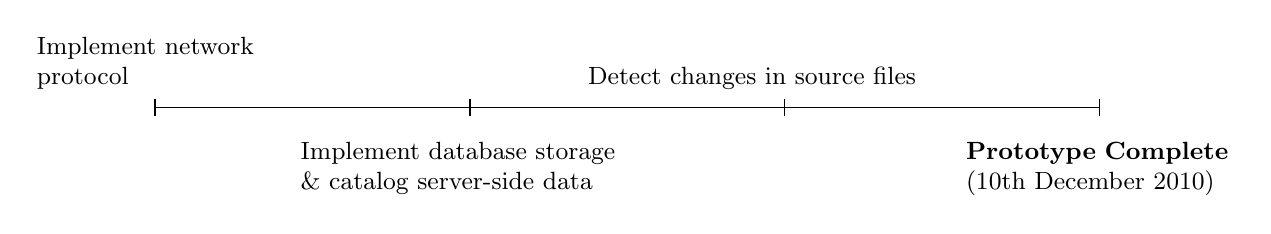
\begin{tikzpicture}
    \tikzstyle{every node}=[font=\small]
    \draw (0,0) -- (12,0);

    \draw (0cm,3pt) -- (0cm,-3pt) node[text width=3cm,above=6pt] {Implement
    network protocol};

    \draw (4cm,3pt) -- (4cm,-3pt) node[text width=4.3cm,below=6pt] {Implement
    database storage \& catalog server-side data};

    \draw (8cm,3pt) -- (8cm,-3pt) node[text width=5cm,above=6pt] {Detect
    changes in source files};

    \draw (12cm,3pt) -- (12cm,-3pt) node[text width=3.4cm,below=6pt]
    {\textbf{Prototype Complete} (10th December 2010)};

\end{tikzpicture}
\]

\[ 
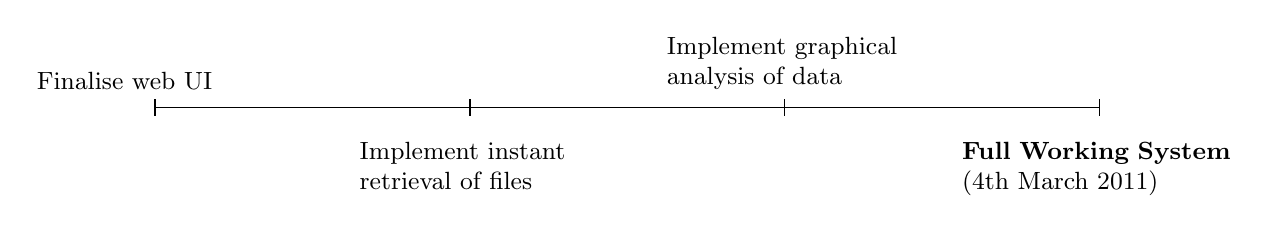
\begin{tikzpicture}
    \tikzstyle{every node}=[font=\small]
    \draw (0,0) -- (12,0);

    \draw (0cm,3pt) -- (0cm,-3pt) node[text width=3cm,above=6pt] {Finalise web
    UI};

    \draw (4cm,3pt) -- (4cm,-3pt) node[text width=2.8cm,below=6pt] {Implement
    instant retrieval of files};

    \draw (8cm,3pt) -- (8cm,-3pt) node[text width=3cm,above=6pt] {Implement
    graphical analysis of data};

    \draw (12cm,3pt) -- (12cm,-3pt) node[text width=3.5cm,below=6pt]
    {\textbf{Full Working System} (4th March 2011)};

\end{tikzpicture}
\]

\[ 

\begin{tikzpicture}
    \tikzstyle{every node}=[font=\small]
    \draw (0,0) -- (12,0);

    \draw (0cm,3pt) -- (0cm,-3pt) node[text width=3.4cm,above=6pt] {Construct
    testing plan};

    \draw (4cm,3pt) -- (4cm,-3pt) node[text width=3cm,below=6pt] {Implement
    unit tests};

    \draw (8cm,3pt) -- (8cm,-3pt) node[text width=3.6cm,above=6pt] {Write up
    testing results \& evaluate system};

    \draw (12cm,3pt) -- (12cm,-3pt) node[text width=5.3cm,below=6pt]
    {\textbf{Testing \& Evaluation Complete} (25th March 2011)};

\end{tikzpicture}
\]

\[ 

\begin{tikzpicture}
    \tikzstyle{every node}=[font=\small]
    \draw (0,0) -- (12,0);

    \draw (0cm,3pt) -- (0cm,-3pt) node[text width=3cm,above=6pt] {Project plan};

    \draw (3cm,3pt) -- (3cm,-3pt) node[text width=2cm,below=6pt] {Presentation};

    \draw (6cm,3pt) -- (6cm,-3pt) node[text width=2.2cm,above=6pt] {Sample
    chapter};

    \draw (9cm,3pt) -- (9cm,-3pt) node[text width=0.8cm,below=6pt] {Draft};

    \draw (12cm,3pt) -- (12cm,-3pt) node[text width=4.4cm,above=6pt]
    {\textbf{Documentation Complete} (31st April 2010)};

\end{tikzpicture}
\]
\end{flushright}

\end{document}
